\chapter{Análise amortizada}

\index{amortized analysis}

A complexidade de tempo de um algoritmo
é, muitas vezes, fácil de analisar
apenas examinando a estrutura
do algoritmo:
quais laços o algoritmo contém
e quantas vezes os laços são executados.
No entanto, às vezes, uma análise direta
não fornece uma imagem verdadeira da eficiência do algoritmo.

A \key{análise amortizada} pode ser usada para analisar
algoritmos que contêm operações cuja
complexidade de tempo varia.
A ideia é estimar o tempo total usado para
todas essas operações durante a
execução do algoritmo, em vez de focar
em operações individuais.

\section{Método dos dois ponteiros}

\index{two pointers method}

No \key{método dos dois ponteiros},
dois ponteiros são usadas para
iterar pelos valores do vetor.
Ambos os ponteiros podem se mover para uma única direção,
o que garante que o algoritmo funcione de forma eficiente.
A seguir, discutiremos dois problemas que podem ser resolvidos
usando o método de dois ponteiros.

\subsubsection{Soma de subvetor}

Como primeiro exemplo,
considere um problema em que recebemos
um vetor de $n$ inteiros positivos
e uma soma alvo $x$,
e queremos encontrar um subvetor cuja soma seja $x$
ou relatar que não existe tal subvetor.

Por exemplo, o vetor
\begin{center}
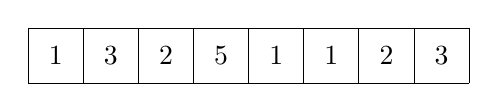
\begin{tikzpicture}[scale=0.7]
\draw (0,0) grid (8,1);

\node at (0.5,0.5) {$1$};
\node at (1.5,0.5) {$3$};
\node at (2.5,0.5) {$2$};
\node at (3.5,0.5) {$5$};
\node at (4.5,0.5) {$1$};
\node at (5.5,0.5) {$1$};
\node at (6.5,0.5) {$2$};
\node at (7.5,0.5) {$3$};
\end{tikzpicture}
\end{center}
contém um subvetor cuja soma é 8:
\begin{center}
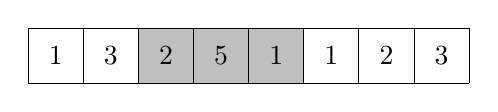
\begin{tikzpicture}[scale=0.7]
\fill[color=lightgray] (2,0) rectangle (5,1);
\draw (0,0) grid (8,1);

\node at (0.5,0.5) {$1$};
\node at (1.5,0.5) {$3$};
\node at (2.5,0.5) {$2$};
\node at (3.5,0.5) {$5$};
\node at (4.5,0.5) {$1$};
\node at (5.5,0.5) {$1$};
\node at (6.5,0.5) {$2$};
\node at (7.5,0.5) {$3$};
\end{tikzpicture}
\end{center}

Este problema pode ser resolvido em
tempo $O(n)$ usando o método de dois ponteiros.
A ideia é manter ponteiros que apontam para o
primeiro e o último valor de um subvetor.
A cada turno, o ponteiro esquerdo se move um passo
para a direita e o ponteiro direito se move para a direita
enquanto a soma do subvetor resultante for no máximo $x$.
Se a soma se tornar exatamente $x$,
uma solução foi encontrada.

Como exemplo, considere o seguinte vetor
e uma soma alvo $x=8$:
\begin{center}
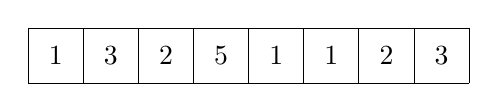
\begin{tikzpicture}[scale=0.7]
\draw (0,0) grid (8,1);

\node at (0.5,0.5) {$1$};
\node at (1.5,0.5) {$3$};
\node at (2.5,0.5) {$2$};
\node at (3.5,0.5) {$5$};
\node at (4.5,0.5) {$1$};
\node at (5.5,0.5) {$1$};
\node at (6.5,0.5) {$2$};
\node at (7.5,0.5) {$3$};
\end{tikzpicture}
\end{center}

O subvetor inicial contém os valores
1, 3 e 2, cuja soma é 6:

\begin{center}
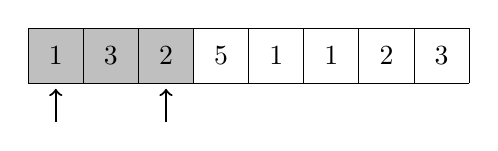
\begin{tikzpicture}[scale=0.7]
\fill[color=lightgray] (0,0) rectangle (3,1);
\draw (0,0) grid (8,1);

\node at (0.5,0.5) {$1$};
\node at (1.5,0.5) {$3$};
\node at (2.5,0.5) {$2$};
\node at (3.5,0.5) {$5$};
\node at (4.5,0.5) {$1$};
\node at (5.5,0.5) {$1$};
\node at (6.5,0.5) {$2$};
\node at (7.5,0.5) {$3$};

\draw[thick,->] (0.5,-0.7) -- (0.5,-0.1);
\draw[thick,->] (2.5,-0.7) -- (2.5,-0.1);
\end{tikzpicture}
\end{center}

Então, o ponteiro esquerdo se move um passo para a direita.
O ponteiro direito não se move, porque, caso contrário,
a soma do subvetor excederia $x$.

\begin{center}
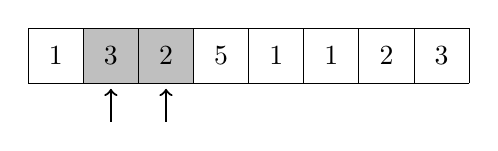
\begin{tikzpicture}[scale=0.7]
\fill[color=lightgray] (1,0) rectangle (3,1);
\draw (0,0) grid (8,1);

\node at (0.5,0.5) {$1$};
\node at (1.5,0.5) {$3$};
\node at (2.5,0.5) {$2$};
\node at (3.5,0.5) {$5$};
\node at (4.5,0.5) {$1$};
\node at (5.5,0.5) {$1$};
\node at (6.5,0.5) {$2$};
\node at (7.5,0.5) {$3$};

\draw[thick,->] (1.5,-0.7) -- (1.5,-0.1);
\draw[thick,->] (2.5,-0.7) -- (2.5,-0.1);
\end{tikzpicture}
\end{center}

Novamente, o ponteiro esquerdo se move um passo para a direita,
e desta vez o ponteiro direito se move três
passos para a direita.
A soma do subvetor é $2+5+1=8$, então um subvetor
cuja soma é $x$ foi encontrado.

\begin{center}
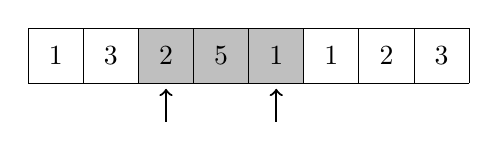
\begin{tikzpicture}[scale=0.7]
\fill[color=lightgray] (2,0) rectangle (5,1);
\draw (0,0) grid (8,1);

\node at (0.5,0.5) {$1$};
\node at (1.5,0.5) {$3$};
\node at (2.5,0.5) {$2$};
\node at (3.5,0.5) {$5$};
\node at (4.5,0.5) {$1$};
\node at (5.5,0.5) {$1$};
\node at (6.5,0.5) {$2$};
\node at (7.5,0.5) {$3$};

\draw[thick,->] (2.5,-0.7) -- (2.5,-0.1);
\draw[thick,->] (4.5,-0.7) -- (4.5,-0.1);
\end{tikzpicture}
\end{center}

O tempo de execução do algoritmo depende de
o número de passos que o ponteiro direito se move.
Embora não haja um limite superior útil sobre quantos passos o
ponteiro pode se mover em um \emph{único} turno.
sabemos que o ponteiro se move \emph{um total de}
$O(n)$ passos durante o algoritmo,
porque ela só se move para a direita.

Como o ponteiro esquerdo e o direito
se movem $O(n)$ passos durante o algoritmo,
o algoritmo funciona em tempo $O(n)$.

\subsubsection{Problema 2SUM}

\index{2SUM problem}

Outro problema que pode ser resolvido usando
o método de dois ponteiros é o seguinte problema,
também conhecido como o \key{problema 2SUM}:
dado um vetor de $n$ números e
uma soma alvo $x$, encontre
dois valores do vetor de forma que sua soma seja $x$,
ou relate que tais valores não existem.

Para resolver o problema, primeiro
ordenamos os valores do vetor em ordem crescente.
Depois disso, iteramos pelo vetor usando
dois ponteiros.
O ponteiro esquerdo começa no primeiro valor
e se move um passo para a direita a cada turno.
O ponteiro direito começa no último valor
e sempre se move para a esquerda até que a soma do
ponteiro esquerdo e direita seja no máximo $x$.
Se a soma for exatamente $x$,
uma solução foi encontrada.

Por exemplo, considere o seguinte vetor
e uma soma alvo $x=12$:
\begin{center}
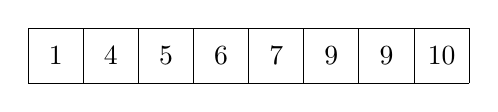
\begin{tikzpicture}[scale=0.7]
\draw (0,0) grid (8,1);

\node at (0.5,0.5) {$1$};
\node at (1.5,0.5) {$4$};
\node at (2.5,0.5) {$5$};
\node at (3.5,0.5) {$6$};
\node at (4.5,0.5) {$7$};
\node at (5.5,0.5) {$9$};
\node at (6.5,0.5) {$9$};
\node at (7.5,0.5) {$10$};
\end{tikzpicture}
\end{center}

As posições iniciais dos ponteiros
são como se segue.
A soma dos valores é $1+10=11$
que é menor que $x$.

\begin{center}
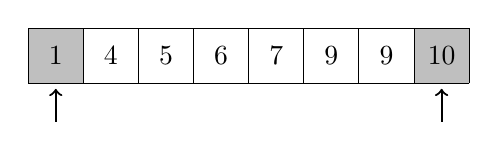
\begin{tikzpicture}[scale=0.7]
\fill[color=lightgray] (0,0) rectangle (1,1);
\fill[color=lightgray] (7,0) rectangle (8,1);
\draw (0,0) grid (8,1);

\node at (0.5,0.5) {$1$};
\node at (1.5,0.5) {$4$};
\node at (2.5,0.5) {$5$};
\node at (3.5,0.5) {$6$};
\node at (4.5,0.5) {$7$};
\node at (5.5,0.5) {$9$};
\node at (6.5,0.5) {$9$};
\node at (7.5,0.5) {$10$};

\draw[thick,->] (0.5,-0.7) -- (0.5,-0.1);
\draw[thick,->] (7.5,-0.7) -- (7.5,-0.1);
\end{tikzpicture}
\end{center}

Então o ponteiro esquerdo se move um passo para a direita.
O ponteiro direito se move três passos para a esquerda,
e a soma se torna $4+7=11$.

\begin{center}
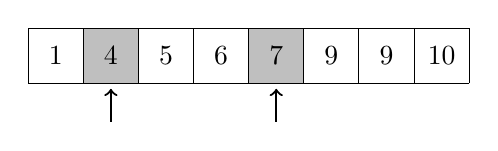
\begin{tikzpicture}[scale=0.7]
\fill[color=lightgray] (1,0) rectangle (2,1);
\fill[color=lightgray] (4,0) rectangle (5,1);
\draw (0,0) grid (8,1);

\node at (0.5,0.5) {$1$};
\node at (1.5,0.5) {$4$};
\node at (2.5,0.5) {$5$};
\node at (3.5,0.5) {$6$};
\node at (4.5,0.5) {$7$};
\node at (5.5,0.5) {$9$};
\node at (6.5,0.5) {$9$};
\node at (7.5,0.5) {$10$};

\draw[thick,->] (1.5,-0.7) -- (1.5,-0.1);
\draw[thick,->] (4.5,-0.7) -- (4.5,-0.1);
\end{tikzpicture}
\end{center}

Depois disso, o ponteiro esquerdo se move um passo para a direita novamente.
O ponteiro direito não se move e uma solução
$5+7=12$ foi encontrada.

\begin{center}
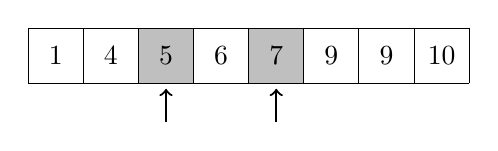
\begin{tikzpicture}[scale=0.7]
\fill[color=lightgray] (2,0) rectangle (3,1);
\fill[color=lightgray] (4,0) rectangle (5,1);
\draw (0,0) grid (8,1);

\node at (0.5,0.5) {$1$};
\node at (1.5,0.5) {$4$};
\node at (2.5,0.5) {$5$};
\node at (3.5,0.5) {$6$};
\node at (4.5,0.5) {$7$};
\node at (5.5,0.5) {$9$};
\node at (6.5,0.5) {$9$};
\node at (7.5,0.5) {$10$};

\draw[thick,->] (2.5,-0.7) -- (2.5,-0.1);
\draw[thick,->] (4.5,-0.7) -- (4.5,-0.1);
\end{tikzpicture}
\end{center}

O tempo de execução do algoritmo é
$O(n \log n)$, pois primeiro ele ordena
o vetor em tempo $O(n \log n)$,
e então ambos os ponteiros movem $O(n)$ passos.

Observe que é possível resolver o problema
de outra forma em tempo $O(n \log n)$ usando a busca binária.
Nessa solução, iteramos pelo vetor
e, para cada valor do vetor, tentamos encontrar outro
valor que produza a soma $x$.
Isso pode ser feito realizando $n$ buscas binárias,
cada uma das quais leva tempo $O(\log n)$.

\index{3SUM problem}
Um problema mais difícil é
o \key{problema 3SUM} que pede para
encontrar \emph{três} valores de vetor
cuja soma seja $x$.
Usando a ideia do algoritmo acima,
este problema pode ser resolvido em tempo $O(n^2)$\footnote{Por muito tempo,
pensou-se que resolver
o problema 3SUM de forma mais eficiente do que em tempo $O(n^2)$
não seria possível.
No entanto, em 2014, descobriu-se \cite{gro14}
que este não é o caso.}.
Você consegue ver como?

\section{Elementos menores mais próximos}

\index{nearest smaller elements}

A análise amortizada é frequentemente usada para
estimar o número de operações
realizadas em uma estrutura de dados.
As operações podem ser distribuídas de forma desigual, de modo que
a maioria das operações ocorra durante uma
determinada fase do algoritmo, mas o número total de
operações é limitado.

Como exemplo, considere o problema
de encontrar para cada elemento do vetor
o \key{elemento menor mais próximo}, ou seja,
o primeiro elemento menor que precede o elemento
no vetor.
É possível que tal elemento não exista,
caso em que o algoritmo deve relatar isso.
A seguir, veremos como o problema pode ser
resolvido de forma eficiente usando uma estrutura de pilha.

Percorremos o vetor da esquerda para a direita
e mantemos uma pilha de elementos do vetor.
Em cada posição do vetor, removemos elementos da pilha
até que o elemento superior seja menor que o
elemento atual, ou a pilha esteja vazia.
Então, relatamos que o elemento superior é
o elemento menor mais próximo do elemento atual,
ou se a pilha estiver vazia, não existe tal elemento.
Finalmente, adicionamos o elemento atual à pilha.

Como exemplo, considere o seguinte vetor:
\begin{center}
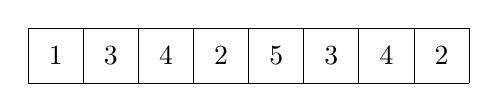
\begin{tikzpicture}[scale=0.7]
\draw (0,0) grid (8,1);

\node at (0.5,0.5) {$1$};
\node at (1.5,0.5) {$3$};
\node at (2.5,0.5) {$4$};
\node at (3.5,0.5) {$2$};
\node at (4.5,0.5) {$5$};
\node at (5.5,0.5) {$3$};
\node at (6.5,0.5) {$4$};
\node at (7.5,0.5) {$2$};
\end{tikzpicture}
\end{center}

Primeiro, os elementos 1, 3 e 4 são adicionados à pilha,
porque cada elemento é maior que o elemento anterior.
Assim, o elemento menor mais próximo de 4 é 3,
e o elemento menor mais próximo de 3 é 1.
\begin{center}
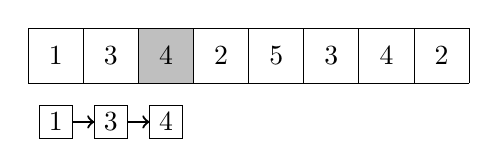
\begin{tikzpicture}[scale=0.7]
\fill[color=lightgray] (2,0) rectangle (3,1);
\draw (0,0) grid (8,1);

\node at (0.5,0.5) {$1$};
\node at (1.5,0.5) {$3$};
\node at (2.5,0.5) {$4$};
\node at (3.5,0.5) {$2$};
\node at (4.5,0.5) {$5$};
\node at (5.5,0.5) {$3$};
\node at (6.5,0.5) {$4$};
\node at (7.5,0.5) {$2$};

\draw (0.2,0.2-1.2) rectangle (0.8,0.8-1.2);
\draw (1.2,0.2-1.2) rectangle (1.8,0.8-1.2);
\draw (2.2,0.2-1.2) rectangle (2.8,0.8-1.2);

\node at (0.5,0.5-1.2) {$1$};
\node at (1.5,0.5-1.2) {$3$};
\node at (2.5,0.5-1.2) {$4$};

\draw[->,thick] (0.8,0.5-1.2) -- (1.2,0.5-1.2);
\draw[->,thick] (1.8,0.5-1.2) -- (2.2,0.5-1.2);
\end{tikzpicture}
\end{center}

O próximo elemento 2 é menor que os dois principais
elementos na pilha.
Assim, os elementos 3 e 4 são removidos da pilha,
e então o elemento 2 é adicionado à pilha.
Seu elemento menor mais próximo é 1:
\begin{center}
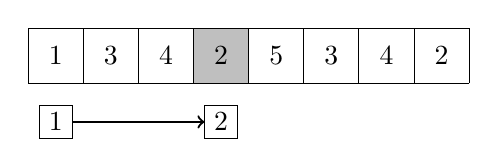
\begin{tikzpicture}[scale=0.7]
\fill[color=lightgray] (3,0) rectangle (4,1);
\draw (0,0) grid (8,1);

\node at (0.5,0.5) {$1$};
\node at (1.5,0.5) {$3$};
\node at (2.5,0.5) {$4$};
\node at (3.5,0.5) {$2$};
\node at (4.5,0.5) {$5$};
\node at (5.5,0.5) {$3$};
\node at (6.5,0.5) {$4$};
\node at (7.5,0.5) {$2$};

\draw (0.2,0.2-1.2) rectangle (0.8,0.8-1.2);
\draw (3.2,0.2-1.2) rectangle (3.8,0.8-1.2);

\node at (0.5,0.5-1.2) {$1$};
\node at (3.5,0.5-1.2) {$2$};

\draw[->,thick] (0.8,0.5-1.2) -- (3.2,0.5-1.2);
\end{tikzpicture}
\end{center}

Então, o elemento 5 é maior que o elemento 2,
então ele será adicionado à pilha, e
seu elemento menor mais próximo é 2:
\begin{center}
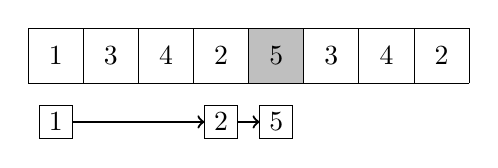
\begin{tikzpicture}[scale=0.7]
\fill[color=lightgray] (4,0) rectangle (5,1);
\draw (0,0) grid (8,1);

\node at (0.5,0.5) {$1$};
\node at (1.5,0.5) {$3$};
\node at (2.5,0.5) {$4$};
\node at (3.5,0.5) {$2$};
\node at (4.5,0.5) {$5$};
\node at (5.5,0.5) {$3$};
\node at (6.5,0.5) {$4$};
\node at (7.5,0.5) {$2$};

\draw (0.2,0.2-1.2) rectangle (0.8,0.8-1.2);
\draw (3.2,0.2-1.2) rectangle (3.8,0.8-1.2);
\draw (4.2,0.2-1.2) rectangle (4.8,0.8-1.2);

\node at (0.5,0.5-1.2) {$1$};
\node at (3.5,0.5-1.2) {$2$};
\node at (4.5,0.5-1.2) {$5$};

\draw[->,thick] (0.8,0.5-1.2) -- (3.2,0.5-1.2);
\draw[->,thick] (3.8,0.5-1.2) -- (4.2,0.5-1.2);
\end{tikzpicture}
\end{center}

Depois disso, o elemento 5 é removido da pilha
e os elementos 3 e 4 são adicionados à pilha:
\begin{center}
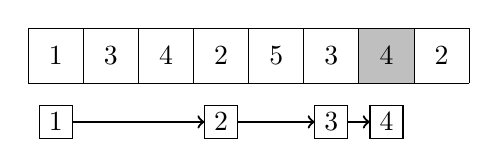
\begin{tikzpicture}[scale=0.7]
\fill[color=lightgray] (6,0) rectangle (7,1);
\draw (0,0) grid (8,1);

\node at (0.5,0.5) {$1$};
\node at (1.5,0.5) {$3$};
\node at (2.5,0.5) {$4$};
\node at (3.5,0.5) {$2$};
\node at (4.5,0.5) {$5$};
\node at (5.5,0.5) {$3$};
\node at (6.5,0.5) {$4$};
\node at (7.5,0.5) {$2$};

\draw (0.2,0.2-1.2) rectangle (0.8,0.8-1.2);
\draw (3.2,0.2-1.2) rectangle (3.8,0.8-1.2);
\draw (5.2,0.2-1.2) rectangle (5.8,0.8-1.2);
\draw (6.2,0.2-1.2) rectangle (6.8,0.8-1.2);

\node at (0.5,0.5-1.2) {$1$};
\node at (3.5,0.5-1.2) {$2$};
\node at (5.5,0.5-1.2) {$3$};
\node at (6.5,0.5-1.2) {$4$};

\draw[->,thick] (0.8,0.5-1.2) -- (3.2,0.5-1.2);
\draw[->,thick] (3.8,0.5-1.2) -- (5.2,0.5-1.2);
\draw[->,thick] (5.8,0.5-1.2) -- (6.2,0.5-1.2);
\end{tikzpicture}
\end{center}

Finalmente, todos os elementos, exceto 1, são removidos
da pilha e o último elemento 2
é adicionado à pilha:

\begin{center}
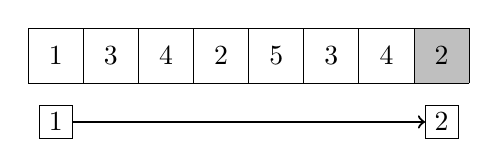
\begin{tikzpicture}[scale=0.7]
\fill[color=lightgray] (7,0) rectangle (8,1);
\draw (0,0) grid (8,1);

\node at (0.5,0.5) {$1$};
\node at (1.5,0.5) {$3$};
\node at (2.5,0.5) {$4$};
\node at (3.5,0.5) {$2$};
\node at (4.5,0.5) {$5$};
\node at (5.5,0.5) {$3$};
\node at (6.5,0.5) {$4$};
\node at (7.5,0.5) {$2$};

\draw (0.2,0.2-1.2) rectangle (0.8,0.8-1.2);
\draw (7.2,0.2-1.2) rectangle (7.8,0.8-1.2);

\node at (0.5,0.5-1.2) {$1$};
\node at (7.5,0.5-1.2) {$2$};

\draw[->,thick] (0.8,0.5-1.2) -- (7.2,0.5-1.2);
\end{tikzpicture}
\end{center}

A eficiência do algoritmo depende de
o número total de operações de pilha.
Se o elemento atual for maior que
o elemento superior na pilha, ele é diretamente
adicionado à pilha, o que é eficiente.
No entanto, às vezes a pilha pode conter vários
elementos maiores e leva tempo para removê-los.
Ainda assim, cada elemento é adicionado \emph{exatamente uma vez} à pilha
e removido \emph{no máximo uma vez} da pilha.
Assim, cada elemento causa $O(1)$ operações de pilha,
e o algoritmo funciona em tempo $O(n)$.
\section{Mínimo da janela deslizante}

\index{janela deslizante}
\index{mínimo da janela deslizante}

Uma \key{janela deslizante} é um subvetor de tamanho constante
que se move da esquerda para a direita através do vetor.
Em cada posição da janela,
queremos calcular alguma informação
sobre os elementos dentro da janela.
Nesta seção, vamos focar no problema
de manter o \key{mínimo da janela deslizante},
o que significa que
devemos reportar o menor valor dentro de cada janela.

O mínimo da janela deslizante pode ser calculado
usando uma ideia semelhante à que usamos para calcular
os elementos menores mais próximos.
Mantemos uma fila
onde cada elemento é maior que
o elemento anterior,
e o primeiro elemento
sempre corresponde ao elemento mínimo dentro da janela.
Após cada movimento da janela,
removemos elementos do final da fila
até que o último elemento da fila
seja menor que o novo elemento da janela,
ou a fila fique vazia.
Também removemos o primeiro elemento da fila
se ele não estiver mais dentro da janela.
Finalmente, adicionamos o novo elemento da janela
ao final da fila.

Como exemplo, considere o seguinte vetor:

\begin{center}
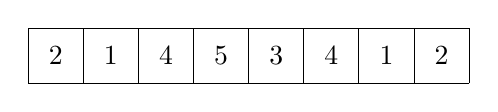
\begin{tikzpicture}[scale=0.7]
\draw (0,0) grid (8,1);

\node at (0.5,0.5) {$2$};
\node at (1.5,0.5) {$1$};
\node at (2.5,0.5) {$4$};
\node at (3.5,0.5) {$5$};
\node at (4.5,0.5) {$3$};
\node at (5.5,0.5) {$4$};
\node at (6.5,0.5) {$1$};
\node at (7.5,0.5) {$2$};
\end{tikzpicture}
\end{center}

Suponha que o tamanho da janela deslizante seja 4.
Na primeira posição da janela, o menor valor é 1:
\begin{center}
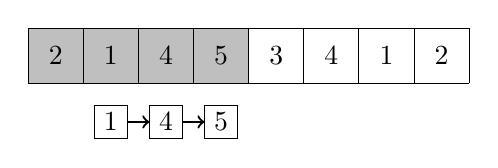
\begin{tikzpicture}[scale=0.7]
\fill[color=lightgray] (0,0) rectangle (4,1);
\draw (0,0) grid (8,1);

\node at (0.5,0.5) {$2$};
\node at (1.5,0.5) {$1$};
\node at (2.5,0.5) {$4$};
\node at (3.5,0.5) {$5$};
\node at (4.5,0.5) {$3$};
\node at (5.5,0.5) {$4$};
\node at (6.5,0.5) {$1$};
\node at (7.5,0.5) {$2$};

\draw (1.2,0.2-1.2) rectangle (1.8,0.8-1.2);
\draw (2.2,0.2-1.2) rectangle (2.8,0.8-1.2);
\draw (3.2,0.2-1.2) rectangle (3.8,0.8-1.2);

\node at (1.5,0.5-1.2) {$1$};
\node at (2.5,0.5-1.2) {$4$};
\node at (3.5,0.5-1.2) {$5$};

\draw[->,thick] (1.8,0.5-1.2) -- (2.2,0.5-1.2);
\draw[->,thick] (2.8,0.5-1.2) -- (3.2,0.5-1.2);
\end{tikzpicture}
\end{center}

Então a janela se move um passo para a direita.
O novo elemento 3 é menor que os elementos
4 e 5 na fila, então os elementos 4 e 5
são removidos da fila
e o elemento 3 é adicionado à fila.
O menor valor ainda é 1.
\begin{center}
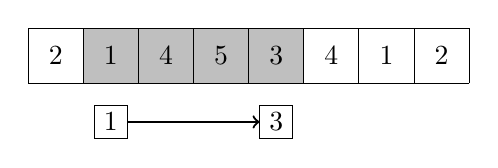
\begin{tikzpicture}[scale=0.7]
\fill[color=lightgray] (1,0) rectangle (5,1);
\draw (0,0) grid (8,1);

\node at (0.5,0.5) {$2$};
\node at (1.5,0.5) {$1$};
\node at (2.5,0.5) {$4$};
\node at (3.5,0.5) {$5$};
\node at (4.5,0.5) {$3$};
\node at (5.5,0.5) {$4$};
\node at (6.5,0.5) {$1$};
\node at (7.5,0.5) {$2$};

\draw (1.2,0.2-1.2) rectangle (1.8,0.8-1.2);
\draw (4.2,0.2-1.2) rectangle (4.8,0.8-1.2);

\node at (1.5,0.5-1.2) {$1$};
\node at (4.5,0.5-1.2) {$3$};

\draw[->,thick] (1.8,0.5-1.2) -- (4.2,0.5-1.2);
\end{tikzpicture}
\end{center}

Depois disso, a janela se move novamente,
e o menor elemento 1
não pertence mais à janela.
Assim, ele é removido da fila e o menor
valor agora é 3. Além disso, o novo elemento 4
é adicionado à fila.
\begin{center}
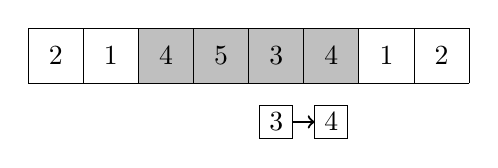
\begin{tikzpicture}[scale=0.7]
\fill[color=lightgray] (2,0) rectangle (6,1);
\draw (0,0) grid (8,1);

\node at (0.5,0.5) {$2$};
\node at (1.5,0.5) {$1$};
\node at (2.5,0.5) {$4$};
\node at (3.5,0.5) {$5$};
\node at (4.5,0.5) {$3$};
\node at (5.5,0.5) {$4$};
\node at (6.5,0.5) {$1$};
\node at (7.5,0.5) {$2$};

\draw (4.2,0.2-1.2) rectangle (4.8,0.8-1.2);
\draw (5.2,0.2-1.2) rectangle (5.8,0.8-1.2);

\node at (4.5,0.5-1.2) {$3$};
\node at (5.5,0.5-1.2) {$4$};

\draw[->,thick] (4.8,0.5-1.2) -- (5.2,0.5-1.2);
\end{tikzpicture}
\end{center}

O próximo novo elemento 1 é menor que todos os elementos
na fila.
Assim, todos os elementos são removidos da fila
e ela conterá apenas o elemento 1:
\begin{center}
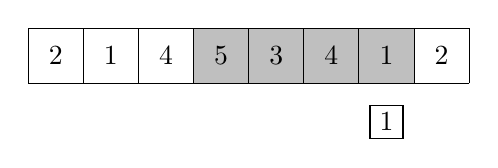
\begin{tikzpicture}[scale=0.7]
\fill[color=lightgray] (3,0) rectangle (7,1);
\draw (0,0) grid (8,1);

\node at (0.5,0.5) {$2$};
\node at (1.5,0.5) {$1$};
\node at (2.5,0.5) {$4$};
\node at (3.5,0.5) {$5$};
\node at (4.5,0.5) {$3$};
\node at (5.5,0.5) {$4$};
\node at (6.5,0.5) {$1$};
\node at (7.5,0.5) {$2$};

\draw (6.2,0.2-1.2) rectangle (6.8,0.8-1.2);

\node at (6.5,0.5-1.2) {$1$};
\end{tikzpicture}
\end{center}

Finalmente, a janela atinge sua última posição.
O elemento 2 é adicionado à fila,
mas o menor valor dentro da janela
ainda é 1.
\begin{center}
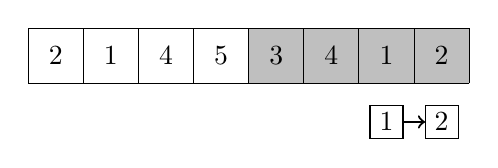
\begin{tikzpicture}[scale=0.7]
\fill[color=lightgray] (4,0) rectangle (8,1);
\draw (0,0) grid (8,1);

\node at (0.5,0.5) {$2$};
\node at (1.5,0.5) {$1$};
\node at (2.5,0.5) {$4$};
\node at (3.5,0.5) {$5$};
\node at (4.5,0.5) {$3$};
\node at (5.5,0.5) {$4$};
\node at (6.5,0.5) {$1$};
\node at (7.5,0.5) {$2$};

\draw (6.2,0.2-1.2) rectangle (6.8,0.8-1.2);
\draw (7.2,0.2-1.2) rectangle (7.8,0.8-1.2);

\node at (6.5,0.5-1.2) {$1$};
\node at (7.5,0.5-1.2) {$2$};

\draw[->,thick] (6.8,0.5-1.2) -- (7.2,0.5-1.2);
\end{tikzpicture}
\end{center}

Como cada elemento do vetor
é adicionado à fila exatamente uma vez e
removido da fila no máximo uma vez,
o algoritmo funciona em tempo $O(n)$.
